\documentclass{article}
\usepackage[english, russian]{babel}
\usepackage[utf8]{inputenc}
\usepackage{hyphenat}
\usepackage{amsmath}
\usepackage{ amssymb }
\usepackage{amsfonts}
\usepackage{verbatim}
\usepackage{fancyvrb} % \begin{Verbatim}[tabsize=4]
\usepackage{ textcomp }
\usepackage{graphicx}
\graphicspath{ {./images/} }
\usepackage{ upgreek }
\usepackage[a4paper, top=3cm, bottom=2cm, left=1.5cm, right=1cm]{geometry}
\usepackage{array}
\usepackage[T2A]{fontenc}
\usepackage[koi8-r]{inputenc}
\usepackage[usenames.dvipsnames]{color}
\usepackage{alltt}
\usepackage{ stmaryrd }
\linespread{2}
\usepackage{ dsfont }
\usepackage{array}
\usepackage{tikz}
\usetikzlibrary{datavisualization}
\usetikzlibrary{datavisualization.formats.functions}
\usepackage{hyperref}
\usepackage{algorithm}
\usepackage{algpseudocode}
\usepackage{listings}
\usepackage{indentfirst}


%Define the listing package
\usepackage{listings} %code highlighter
\usepackage{color} %use color
\definecolor{mygreen}{rgb}{0,0.6,0}
\definecolor{mygray}{rgb}{0.5,0.5,0.5}
\definecolor{mymauve}{rgb}{0.58,0,0.82}
 
%Customize a bit the look
\lstset{ %
backgroundcolor=\color{white}, % choose the background color; you must add \usepackage{color} or \usepackage{xcolor}
basicstyle=\footnotesize, % the size of the fonts that are used for the code
breakatwhitespace=false, % sets if automatic breaks should only happen at whitespace
breaklines=true, % sets automatic line breaking
captionpos=b, % sets the caption-position to bottom
commentstyle=\color{mygreen}, % comment style
deletekeywords={...}, % if you want to delete keywords from the given language
escapeinside={\%*}{*)}, % if you want to add LaTeX within your code
extendedchars=true, % lets you use non-ASCII characters; for 8-bits encodings only, does not work with UTF-8
frame=single, % adds a frame around the code
keepspaces=true, % keeps spaces in text, useful for keeping indentation of code (possibly needs columns=flexible)
keywordstyle=\color{blue}, % keyword style
% language=Octave, % the language of the code
morekeywords={*,...}, % if you want to add more keywords to the set
numbers=left, % where to put the line-numbers; possible values are (none, left, right)
numbersep=5pt, % how far the line-numbers are from the code
numberstyle=\tiny\color{mygray}, % the style that is used for the line-numbers
rulecolor=\color{black}, % if not set, the frame-color may be changed on line-breaks within not-black text (e.g. comments (green here))
showspaces=false, % show spaces everywhere adding particular underscores; it overrides 'showstringspaces'
showstringspaces=false, % underline spaces within strings only
showtabs=false, % show tabs within strings adding particular underscores
stepnumber=1, % the step between two line-numbers. If it's 1, each line will be numbered
stringstyle=\color{mymauve}, % string literal style
tabsize=2, % sets default tabsize to 2 spaces
title=\lstname % show the filename of files included with \lstinputlisting; also try caption instead of title
}
%END of listing package%
 
\definecolor{darkgray}{rgb}{.4,.4,.4}
\definecolor{purple}{rgb}{0.65, 0.12, 0.82}
 
%define Javascript language
\lstdefinelanguage{JavaScript}{
keywords={typeof, new, true, false, catch, function, return, null, catch, switch, var, if, in, while, do, else, case, break},
keywordstyle=\color{blue}\bfseries,
ndkeywords={class, export, boolean, throw, implements, import, this},
ndkeywordstyle=\color{darkgray}\bfseries,
identifierstyle=\color{black},
sensitive=false,
comment=[l]{//},
morecomment=[s]{/*}{*/},
commentstyle=\color{purple}\ttfamily,
stringstyle=\color{red}\ttfamily,
morestring=[b]',
morestring=[b]"
}
 
\lstset{
language=JavaScript,
extendedchars=true,
basicstyle=\footnotesize\ttfamily,
showstringspaces=false,
showspaces=false,
numbers=left,
numberstyle=\footnotesize,
numbersep=9pt,
tabsize=2,
breaklines=true,
showtabs=false,
captionpos=b
}



\newcommand\tab[1][1cm]{\hspace*{#1}}
\newcommand\pa{\partial}
\newcommand\tb{\textbullet}

\usetikzlibrary{arrows.meta}




\title{Министерство науки и высшего образования Российской Федерации
Федеральное государственное автономное образовательное учреждение высшего образования 
«Национальный исследовательский университет ИТМО»

Факультет Программной инженерии и компьютерной техники
}

\date{09.03.2024}

\begin{document}
\renewcommand{\labelenumii}{\arabic{enumi}.\arabic{enumii}}
\renewcommand{\labelenumiii}{\arabic{enumi}.\arabic{enumii}.\arabic{enumiii}}
\renewcommand{\labelenumiv}{\arabic{enumi}.\arabic{enumii}.\arabic{enumiii}.\arabic{enumiv}}

\maketitle
\begin{center}
{\huge{Лабораторная работа \textnumero 1 Основы программной инженерии }}
\\
{\centering{\huge{Вариант 777}}}

\author{Раевский Григорий, группа 3.2}
\end{center}

\setcounter{secnumdepth}{-1}



\tableofcontents
\newpage

\section{Задание}
Вариант \textnumero 777: \href{https://www.ebay.com/}{ebay.com}

Составить список требований, предъявляемых к разрабатываемому веб-сайту (в соответствии с вариантом). Требования должны делиться на следующие категории:
\begin{enumerate}
    \item Функциональные
    \begin{enumerate}
        \item Требования пользователей сайта
        \item Требования владельцев сайта
    \end{enumerate}
    \item Нефункциональные
\end{enumerate}

Требования необходимо оформить в соответствии с шаблонами RUP (документ SRS - Software Requirements Specification). Для каждого из требований нужно указать его атрибуты (в соответствии с методологией RUP), а также оценить и аргументировать приблизительное количество часов, требующихся на реализацию этого требования.

Для функциональных требований нужно составить UML UseCase-диаграммы, описывающие реализующие их прецеденты использования.

\textbf{Отчёт по лабораторной работе должен содержать:}
\begin{enumerate}
    \item Документ SRS, содержащий список требований к сайту
    \item UseCase-диаграммы прецедентов использования, реализующих функциональные требования
    \item Выводы по работе
\end{enumerate}

\textbf{Вопросы к защите лабораторной работы:}
\begin{enumerate}
    \item Методологии разработки ПО. Унифицированный процесс.
    \item Требования и их категоризация. Атрибуты требований.
    \item Язык UML
    \item Прецеденты использования. UseCase-диаграммы - состав, виды связей.
\end{enumerate}


\section{Введение}

\subsection{Цель}

Цель документа - создать описание системы, обуспечивающей работоспособность целового сайта. ebay.com - онлайн аукцион, а позже маркетплейс, содержащий огромное количество как новых, так и б/у товаров в различных категориях. 

\subsection{Технические термины и информация}

\begin{enumerate}
    \item Формат атрибутов требований: [ID, Приоритет, Статус, Трудоемкость в часах, Стабильность, Целевая версия]
    \item ID требований:
    \begin{enumerate}
        \item FRU - Functional Requirement User - функциональное требование системы для пользователя.
        \item FRA - Functional Requirement Admin - функциональное требование системы для администрации.
        \item NFR - Non Functional Requirement - нефункциональное требование системы.
    \end{enumerate}
    \item Бекенд — часть системы, которая на сервере обрабатывает логику, запросы пользователей и предоставляет данные для сайта.
    \item Фронтенд — часть системы, отображающая пользовательский интерфейс.
    \item Java - объектно-ориентированный строго типизированный язык программирования. 
    \item Python - язык программирования с динамической типизацией.
    \item Oracle Database - система управления базами данных.
    \item GitLab - инструмент жизненного цикла, использующийся для контроля версия и развертывания.
    \item HTML - язык разметки документов для просмотра в браузере.
    \item CSS - язык декорирования и описания внешнего вида документов для просмотра в браузере.
    \item JavaScript - язык программирования, который используется для придания интерактивности страницам в браузере.
    \item React - библиотека для JavaScript для разработки пользовательских интерфейсов.
    
\end{enumerate}

\section{Подробная информация о проекте}

\subsection{Возможности системы}

Система должна предоставлять пользователям зарегистрированным (покупатель, продавец) возможность выставлять свои товары на маркетплейс, покупать их, а так же проводить аукционы. Незарегистированные же пользователи могут только просматривать товары.

\subsection{Виды пользователей}
\begin{enumerate}
    \item Незаригистрированный пользователь способен только просматривать товары, доступные на платформе. Он не способен участвовать в аукционах или оформлять заказы. Он так же не может выставлять свои товары на продажу/аукцион.
    \item Зарегистрированный пользователь способен выступать как в роли покупателя, так и в роли продавца. В роли покупателя он может покупать один или несколько товаров с маркетплейса и участвовать в аукционах других пользователей. В роли продавца он может выставлять свои товары на маркетплейс и на аукцион.
    \item Администратор - супер пользователь, который может настраивать алгоритмы поиска, фильтры, временно (или навсегда) блокировать обычных пользователей. Так же администратор занимается размещением и настройкой рекламы. 
\end{enumerate}

\subsection{Рабочая среда}

 Бекенд: Java, Python, Oracle Database, GitLab.

 Фронтенд: HTML, CSS, JavaScript, React.

\subsection{Ограничения}

Ограничением к доступу к сайту должен быть только нестабильный доступ к сети интернет. В ином случае пользователь должен иметь возможность просматривать содержимое сайта или взаимодействовать с ним в зависимости от его роли.

\subsection{Зависимости}

Доступ к веб сайту должен зависеть только от качества интернет соединения. Однако на работу системы могут повлиять факторы, не зависящие от конечного пользователя, например, проблемы у банковских, почтовых или иных систем. Пользователь всегда должен иметь доступ ко всему функционалу системы (если он не заблокирован администратором).

\section{Функциональные требования}

\subsection{Для пользователя}

\begin{enumerate}
    \item Система должна реализовывать пользователям регистрировать аккаунт для сохранения платежных средств, адресов. [FRU1, MUST have, Одобрено, 150, Низкая, 1] 
    \item Система должна реализовывать поиск товаров тегам, категориям. [FRU2, MUST have, Одобрено, 150, Низкая, 1]
    \item Система должна предоставлять пользователю возможность смены данных и восстановления аккаунта. [FRU3, MUST have, Одобрено, 50, Низкая, 1]
    \item Система должна предоставлять пользователю возможность выбора языка во время регистрации. [FRU4, Should have, Предложено, 48, Высокая, 2]
    \item Система должна предоставлять пользователю просматривать товары: фотографии, описание, отзывы. [FRU5, MUST have, Одобрено, 150, Низкая, 1]
    \item Система должна предоставлять зарегистрированному пользователю возможность формировать корзину, список отслеживаемых товаров. [FRU6, MUST have, Одобрено, 50, Средняя, 1]
    \item Система должна предоставлять зарегистрированному пользователю возможность выставлять свои товары на маркетплейс или аукцион. [FRU7, MUST have, Одобрено, 100, Средняя, 1]
    \item Система должна предоставлять пользователю возможность продвигать свои товары на маркетплейсе или аукционе. [FRU8, Should have, Предложено, 56, Низкая, 2]
    \item Система должна предоставлять зарегистрированному пользователю возможность получать уведомления об аукционах и интересующих товарах на основе просмотренных товаров. [FRU9, Should have, Предложено, 56, Высокая, 2]
    \item Система должна предоставлять зарегистрированному пользователю возможность использования 2FA, аутентификации по номеру телефона или электронной почте. [FRU10, MUST have, Одобрено, 56, Средняя, 3]
    \item Система должна позволять зарегистрированному пользователю изменять платежные данные или адреса доставки. [FRU11, MUST have, Одобрено, 100, Низкая, 1] 
    \item Система должна пользовалять зарегистрированному пользователю оставлять отзывы на приобретенные товары. [FRU12, MUST have, Одобрено, 150, Низкая, 1]
    \item Система должна предоставлять зарегистрированному пользователю возможность обращения к службе поддержки прямо на сайте. [FRU13, MUST have, Предложено, 100, Средняя, 2]
\end{enumerate}


\subsection{Для администратора}

\begin{enumerate}
    \item Система должна предоставлять администрации возможность настраивать систему поиска и фильтрации товаров. [FRA1, MUST have, Одобрено,150, Низкая, 1]
    \item Система должна предоставлять администрации возможность ограничивать доступ к учетными записям пользователей (временная и постоянная блокировка). [FRA2, Should have, Предложено, 150, Средняя, 2]
    \item Система должна предоставлять администрации возможность отслеживать посещаемость сайта. [FRA3, MUST have, Одобрено, 48, Высокая, 1]
    \item Система должна предоставлять администрации возможность интеграции рекламы и управления ей. [FRA4, Should have, Предложено, 150, Низкая, 2]
    \item Система должна предоставлять администрации возможность удаления карточки товара. [FRA5, MUST have, Одобрено, 100, Средняя, 1]
\end{enumerate}

\section{Нефункциональные требования}


\subsection{Usability}

\begin{enumerate}
    \item Система должна обеспечивать возможность работы на браузерах Safari 16, Chrome 109, Яндекс Браузер 32 на всех платформах (компьютер, телефон, планшет). [NFR1, MUST have, Одобрено, 48, Низкая, 1]
    \item Система должна иметь простой и понятный интерфейс с одинаковым дизайном. [NFR2, Should have, Отклонено, 150, Низкая, 3]
    \item Система должна обеспечивать должна иметь документацию на английском языке. [NFR3, MUST have, Одобрено, 200, Высокая, 1]
\end{enumerate}

\subsection{Reliability}

\begin{enumerate}
    \item Максимальный простой (система не доступна пользователю) - 100 часов в год. [NFR4, MUST have, Одобрено, 100, Низкая, 2]
    \item Система должна выполнять автоматическое ежедневное резервное копирование данных. [NFR5, MUST have, Одобрено, 48, Средняя, 1]
\end{enumerate}

\subsection{Perfomance}

\begin{enumerate}
    \item Система должна обеспечивать загрузку главной страницы и страницы профиля пользователя не более чем за 3 секунды при скорости соединения 50 Мбит/с. [NFR6, Could have, Предложено, 100, Низкая, 3] 
    \item Система должна обеспечивать обработку не менее 10'000 запросов (загрузка главной страницы, профиля, карточки товара) в минуту. [NFR7, MUST have, Одобрено, 150, Низкая, 3]

\end{enumerate}

\subsection{Quality}

\begin{enumerate}
    \item Система должна автоматически сохранять информацию о важных событиях или ошибках в логи. [NFR8, MUST have, Одобрено, 24, Средняя, 1]
\end{enumerate}

\subsection{Security}

\begin{enumerate}
    \item Система должна иметь защиту от атак DoS, DDoS, SQL инъекций. [NFR9, MUST have, Одобрено, 150, Низкая, 1]
    \item Система должна хранить всю информацию, которую указывают сами пользователи в зашифрованном виде, применяя хеширование SHA-512. [NFR10, Should have, Предложено, 150, Высокая, 2]
\end{enumerate}

\newpage 
\section{Возможные риски}

\subsection{Технические риски}

\begin{center}
\begin{tabular}{ | m{1em} | m{5cm}| m{2cm} | m{2cm} | m{4cm} | m{3cm} | } 
  \hline
  \textnumero & Риск & Тип & Масштаб потерь & Вероятность & Реакция \\ 
  \hline
  1 & Критический отказ серверного оборудования & Технический & Высокий & Незначительня & Восстановление системы \\
  \hline
  2 & Отказ оборудования посредника & Технический & Высокий & Незначительная & Ждать восстановления системы посредника\\
  \hline
  3 & Отказ системы резервного копирования & Технический & Средний & Незначительная & Восстановление системы\\
  \hline
\end{tabular}
\end{center}

\subsection{Ресурсные риски}

\begin{center}
\begin{tabular}{ | m{1em} | m{5cm}| m{2cm} | m{2cm} | m{4cm} | m{3cm} | } 
  \hline
  \textnumero & Риск & Тип & Масштаб потерь & Вероятность & Реакция \\ 
  \hline
  1 & Нехватка финансирования & Ресурсный & Средний & Средняя & Поиск новых финансов \\
  \hline
  2 & Нехватка персонала &
  Ресурсный & Средний & Незначительная & Поиск новых кадров\\
  \hline
  3 & Нехватка времени на разработку системы & Ресурсный & Средний & Значительная & Переработка плана, перерерасчет временных затрат\\
  \hline
\end{tabular}
\end{center}

\subsection{Бизнес риски}

\begin{center}
\begin{tabular}{ | m{1em} | m{5cm}| m{2cm} | m{2cm} | m{4cm} | m{3cm} | } 
  \hline
  \textnumero & Риск & Тип & Масштаб потерь & Вероятность & Реакция \\ 
  \hline
  1 & Недостаточный объем пользователей & Бизнес & Средний & Незначительная & Привлечение новых пользователей \\
  \hline
  2 & Недостаточная конкуретоспособность & Бизнес & Средний & Незначительная & Поиск способов повышения конкуретоспособности\\
  \hline
\end{tabular}
\end{center}

\subsection{Ресурсные риски}

\begin{center}
\begin{tabular}{ | m{1em} | m{5cm}| m{2cm} | m{2cm} | m{4cm} | m{3cm} | } 
  \hline
  \textnumero & Риск & Тип & Масштаб потерь & Вероятность & Реакция \\ 
  \hline
  1 & Нехватка финансирования & Ресурсный & Средний & Средняя & Поиск новых финансов \\
  \hline
  2 & Нехватка персонала &
  Ресурсный & Средний & Незначительная & Поиск новых кадров\\
  \hline
  3 & Нехватка времени на разработку системы & Ресурсный & Средний & Значительная & Переработка плана, перерерасчет временных затрат\\
  \hline
\end{tabular}
\end{center}

\subsection{Политические риски}

\begin{center}
\begin{tabular}{ | m{1em} | m{5cm}| m{2cm} | m{2cm} | m{4cm} | m{3cm} | } 
  \hline
  \textnumero & Риск & Тип & Масштаб потерь & Вероятность & Реакция \\ 
  \hline
  1 & Смена руководства у компании-заказчика & Политический & Значительный & Незначительная & Обсуждение новых деталей договора, поиск решений \\
  \hline
\end{tabular}
\end{center}

\section{UseCase диаграмма}

\begin{center}
    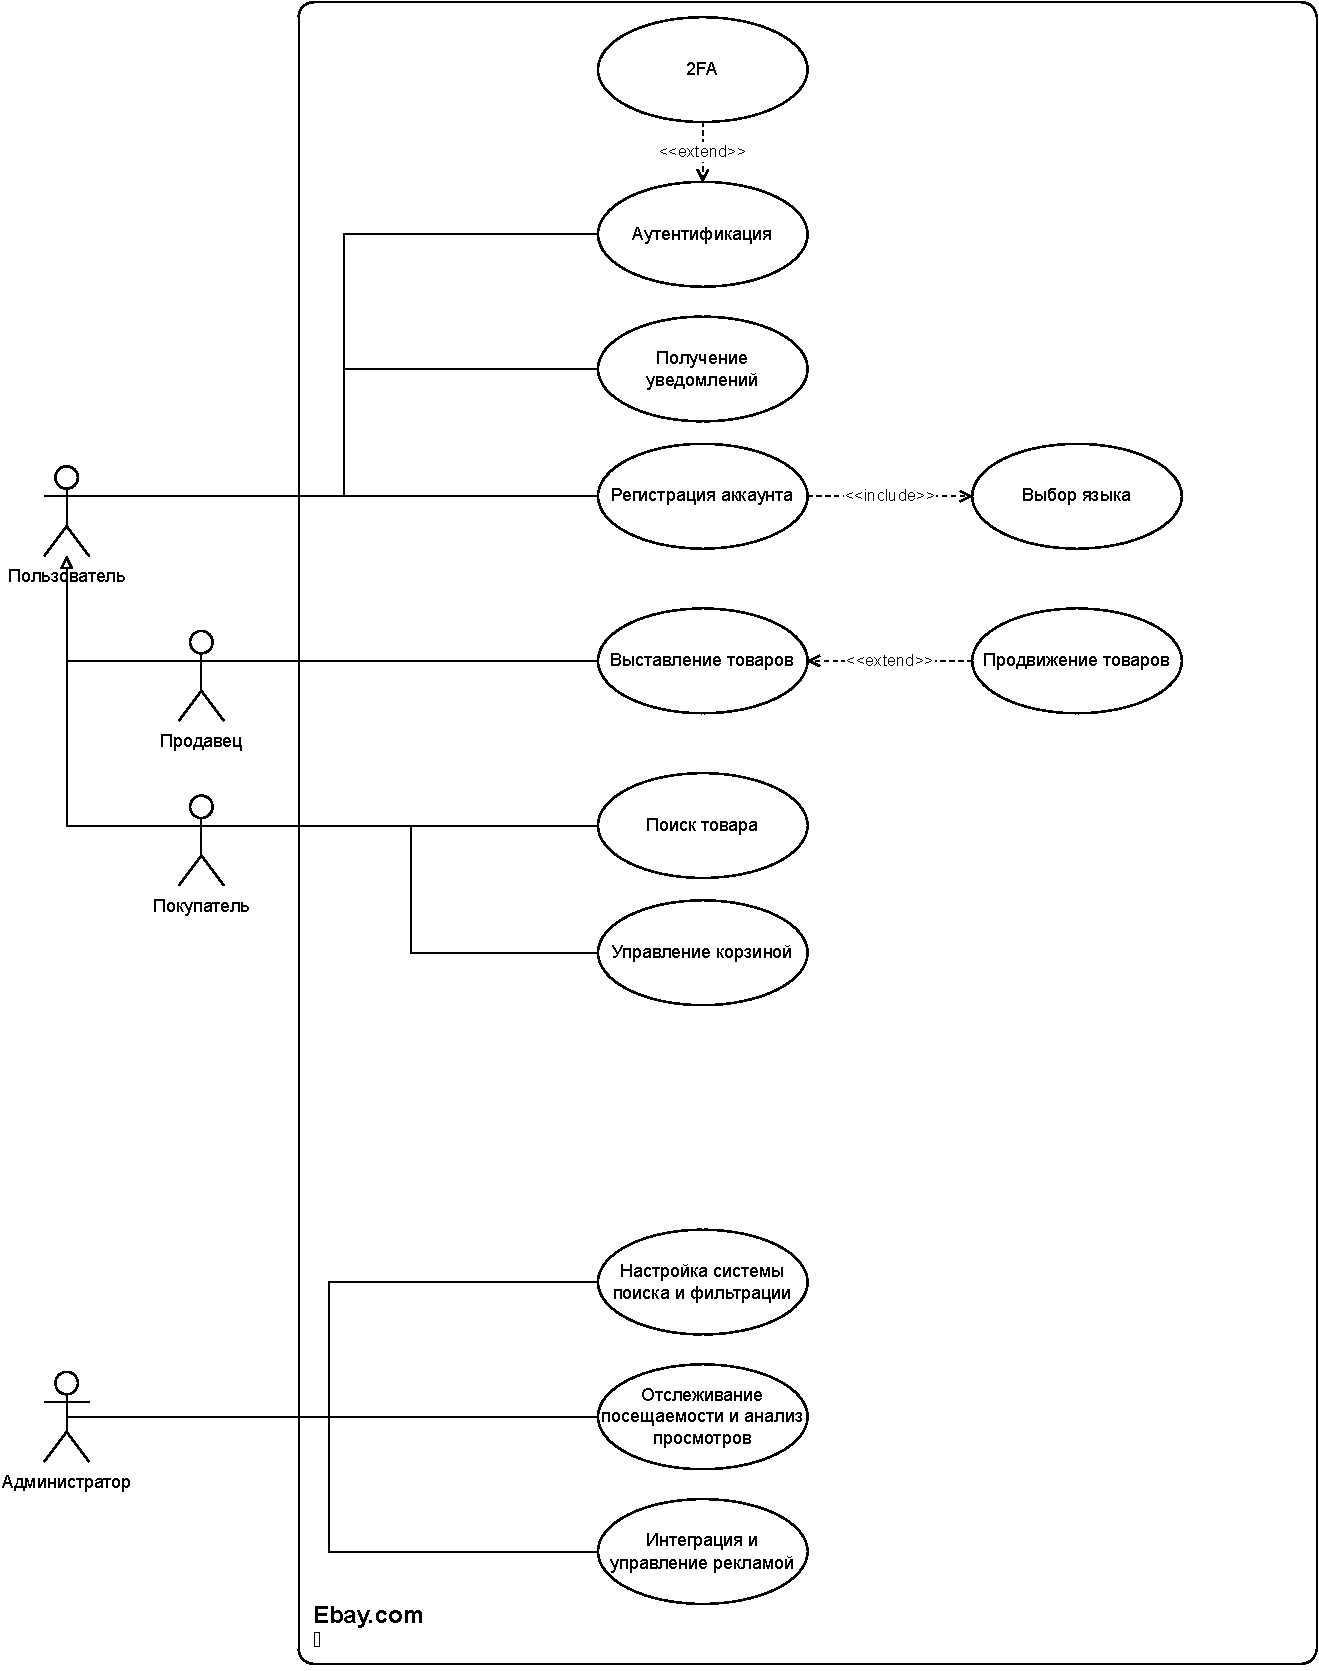
\includegraphics[scale=0.55]{UseCase.drawio.pdf}
\end{center}

\section{Прецеденты}

\subsection{Прецедент 1. Авторизация}
\begin{enumerate}
    \item ID: 1
    \item Краткое описание: Пользователь входит в систему используя свои учетные данные
    \item Главный актер: Пользователь
    \item Предусловия: Пользователь зарегистрирован в системе
    \item Результат: Пользователь вошел в систему и получил доступ к своему аккаунту
    \item Основной поток событий:
    \begin{enumerate}
            \item Пользователь выбирает ввод
            \item Система запрашивает учетные данные (логин и пароль)
            \item Пользователь вводит учетные данные
            \item Система проверяет данные и пользователь получает доступ к системе
    \end{enumerate}
    \item Альтернативный поток событий (для 2FA):
    \begin{enumerate}
            \item После ввода учетных данных (шаг 4) система запрашивает код 2FA
            \item Система проверяет аутентификацию и предоставляет доступ к системе
    \end{enumerate}
    \item Альтернативный поток событий (Восстановление данных аккаунта):
    \begin{enumerate}
            \item После запроса данных от аккаунта (шаг 2) пользователь выбирает опцию восстановления аккаунта
            \item Пользователь указывает свою электронную почту, на которую был зарегистрирован аккаунт
            \item Система находит пользователя, высылает ему на электронную почту код восстановления
            \item Пользователь вводит код восстановления и, при наличии, код 2FA
            \item Система проверяет код восстановления, и, при наличии, код 2FA
            \item Пользователь указывает новые данные аккаунта и входит в него
            \item Система проверяет данные и предоставляет доступ к аккаунту
    \end{enumerate}
\end{enumerate}


\subsection{Прецедент 2. Регистрация аккаунта}
\begin{enumerate}
    \item ID: 2
    \item Краткое описание: Новый пользователь создает аккаунт в системе
    \item Главный актер: Пользователь
    \item Предусловия: У пользователя нет аккаунта
    \item Результат: У пользователя есть аккаунт и он может зайти в систему
    \item Основной поток событий:
    \begin{enumerate}
        \item Пользователь выбирает опцию регистрации
        \item Система запрашивает данные для регистрации
        \item Пользователь вводит нужные данные и выбирает язык интерфейса
        \item Система создает новый аккаунт
        \item Пользователь получает уведомление о регистрации и может пользоваться аккаунтом
    \end{enumerate}
\end{enumerate}


\subsection{Прецедент 3. Поиск товаров}
\begin{enumerate}
    \item ID: 3
    \item Краткое описание: Покупатель ищет товары используя поиск и фильтры системы
    \item Главный актер: Покупатель
    \item Предусловия: Покупатель зашел на сайт
    \item Результат: Система отображает список товаров, которые соответствуют запросу
    \item Основной поток событий:
    \begin{enumerate}
        \item Покупатель заходит на сайт и переходить в раздел поиска товаров
        \item Покупатель вводит ключевое слово в поисковую строку
        \item (Необязательно) Покупатель применяет фильтры 
        \item Система находит товары, удовлетворяющие ключевым словам и фильтрам и формирует список
        \item Система отображает список товаров
        \item Покупатель просматривает список и находит нужный товар
    \end{enumerate}
    \item Альтернативный поток событий (Просмотр конкретного товара):
    \begin{enumerate}
            \item После нахождения нужного товара (шаг 6), пользователь открывает его
            \item Система загружает информацию о товаре (фотографии, описание, отзывы) и предоставляет покупателю
            \item Покупатель просматривает характеристики товара
    \end{enumerate}
\end{enumerate}


\subsection{Прецедент 4. Восстановление данных аккаунта}
\begin{enumerate}
    \item ID: 4
    \item Краткое описание: Покупатель восстанавливает доступ к аккаунту
    \item Главный актер: Покупатель
    \item Предусловия: Покупатель не может войти в аккаунт и желает восстановить к нему доступ
    \item Результат: Доступ к аккаунту востановлен
    \item Основной поток событий:
    \begin{enumerate}
        \item Пользователь выбирает опцию входа в учетную запись 
        \item После запроса данных от аккаунта пользователь выбирает опцию восстановления аккаунта
        \item Пользователь указывает свою электронную почту, на которую был зарегистрирован аккаунт
        \item Система находит пользователя, высылает ему на электронную почту код восстановления
        \item Пользователь вводит код восстановления и, при наличии, код 2FA
        \item Система проверяет код восстановления, и, при наличии, код 2FA
        \item Пользователь указывает новые данные аккаунта и входит в него
        \item Система проверяет данные и предоставляет доступ к аккаунту
    \end{enumerate}
\end{enumerate}

\subsection{Прецедент 5. Обращение к службе поддержки}
\begin{enumerate}
    \item ID: 5
    \item Краткое описание: Пользователь пишет обращение в службу поддержки
    \item Главный актер: Пользователь
    \item Предусловия: Пользователь аутентифицирован
    \item Результат: Пользователь получил ответ от службы поддержки
    \item Основной поток событий:
    \begin{enumerate}
        \item Пользователь выбирает опцию обращения к поддержке в профиле
        \item Пользователь заполняет форму обращения и отправляет ее
        \item Система регистрирует обращение и передает на обработку в службу поддержки
        \item Система получает ответ от службы поддержки, генерирует уведомление и отправляет его пользователю
        \item Пользователь просматривает ответ от службы поддержки
    \end{enumerate}
\end{enumerate}

\subsection{Прецедент 6. Получение уведомлений }
\begin{enumerate}
    \item ID: 6
    \item Краткое описание: Пользователь получает уведомление о важном событии или акции
    \item Главный актер: Пользователь
    \item Предусловия: Пользователь аутентифицирован
    \item Результат: Пользователь получил уведомление
    \item Основной поток событий:
    \begin{enumerate}
        \item Система генерирует уведомление
        \item Уведомление отображается в профиле пользователя и отправляется на почту
        \item Пользователь просматривает уведомление
    \end{enumerate}
\end{enumerate}

\subsection{Прецедент 7. Управление корзиной}
\begin{enumerate}
    \item ID: 7
    \item Краткое описание: Покупатель добавляет, удалять товары в корзину
    \item Главный актер: Покупатель
    \item Предусловия: Покупатель авторизован и нашел интересующий товар
    \item Результат: Товар добавлен в корзину, количество установлено покупателем
    \item Основной поток событий:
    \begin{enumerate}
        \item Покупатель нажимает на кнопку добавления товара в корзину
        \item Система обрабатывает запрос и добавляет 1 единицу товара в корзину
        \item Покупатель переходит в корзину и изменяет количество товара в корзине (при необходимости)
        \item Покупатель может перейти к оформлению заказа
    \end{enumerate}
\end{enumerate}

\subsection{Прецедент 8. Создание отзывов}
\begin{enumerate}
    \item ID: 8
    \item Краткое описание: Покуппатель выбирает полученный товар и пишет к нему отзыв
    \item Главный актер: Покупатель
    \item Предусловия: Покупатель авторизован и у него есть доставленный товар
    \item Результат: Отзыв на странице товара отображается
    \item Основной поток событий:
    \begin{enumerate}
        \item Покупатель открывает раздел заказов в профиле
        \item Покупатель выбирает интересующий товар
        \item Покупатель выбирает опцию добавления отзыва
        \item Покупатель пишет отзыв и отправляет его
        \item Система добавляет отзыв на страницу товара
    \end{enumerate}
\end{enumerate}

\subsection{Прецедент 9. Выставление товаров}
\begin{enumerate}
    \item ID: 9
    \item Краткое описание: Продавец выставляет товар на аукцион или маркетплейс
    \item Главный актер: Продавец
    \item Предусловия: Пользователь аутентифицирован и является продавцом
    \item Результат: Товар выставлен на продажу
    \item Основной поток событий:
    \begin{enumerate}
        \item Продавец выбирает опцию добавления товара
        \item Система запрашивает информацию о товаре
        \item Продавец заполняет информацию о товаре и подтверждает добавление товара
        \item Система публикует товар на площадке
    \end{enumerate}
    Альтернативный поток событий (используется продвижение товаров):
    \begin{enumerate}
        \item После шага 4 основного потока продавец выбирает опцию продвижения товара
        \item Система предлагает варианты продвижения
        \item Продавец выбирает вариант и подтверждает его
        \item Система активирует продвижение
    \end{enumerate}
\end{enumerate}

\subsection{Прецедент 10. Продвижение товаров}
\begin{enumerate}
    \item ID: 10
    \item Краткое описание: Продавец использует систему для продвижения своих товаров в поиске
    \item Главный актер: Продавец
    \item Предусловия: Продавец аутентифицирован и он выставил товары на продажу
    \item Результат: Товар получает дополнительные просмотры на площадке
    \item Основной поток событий:
    \begin{enumerate}
        \item Продавец выбирает товар для продвижения
        \item Система предлагает различные опции для продвижения и их стоимость
        \item Продавец выбирает желаемый вариант и оплачивает его
        \item Система активирует продвижение товара
    \end{enumerate}
\end{enumerate}

\subsection{Прецедент 11. Блокировка пользователя}
\begin{enumerate}
    \item ID: 11
    \item Краткое описание: Администратор  временно или навсегда блокирует пользователя на платформе
    \item Главный актер: Администратор
    \item Предусловия: Администратор зашел в панель управления 
    \item Результат: Специфичный пользователь заблокирован
    \item Основной поток событий:
    \begin{enumerate}
        \item Администратор переходит в раздел управления рекламой
        \item Администратор выбирает определенного пользователя
        \item Администратор настраивает параметры блокировки
        \item Администратор отправил данные о блокировке в систему
        \item Система обработала запрос, заблокировала пользователя
    \end{enumerate}
\end{enumerate}


\subsection{Прецедент 12. Настройка поиска и фильтров}
\begin{enumerate}
    \item ID: 12
    \item Краткое описание: Администратор настраивает и обновляет параметры системы поиска и фильтрации для оптимизации
    \item Главный актер: Администратор
    \item Предусловия: Администратор открыл панель управления
    \item Результат: Система фильтрации улучшена
    \item Основной поток событий:
    \begin{enumerate}
        \item Администратор добавляет новый фильтр, вписывая его описание и значения. 
        \item Администратор изменяет другие фильтры и настройки поиска.
        \item Администратор сохраняет изменения, они обновляются в системе
    \end{enumerate}
\end{enumerate}

\subsection{Прецедент 13. Отслеживание посещаемости}
\begin{enumerate}
    \item ID: 13
    \item Краткое описание: Администратор отслеживает статистику посещаемости сайта
    \item Главный актер: Администратор
    \item Предусловия: Администратор зашел в панель управления
    \item Результат: Администратор просмотрел статистику по сайту за определенный период
    \item Основной поток событий:
    \begin{enumerate}
        \item Администратор переходит в раздел статистики в панели управления
        \item Администратор выбирает промежуток времени для просмотра статистики
        \item Система подгружает данные за заданный период, строит графики и отображает информацию
        \item Администратор просматривает данные и принимает какие-либо решения
    \end{enumerate}
\end{enumerate}

\subsection{Прецедент 14. Интеграция и управление рекламой}
\begin{enumerate}
    \item ID: 14
    \item Краткое описание: Администратор  управляет рекламой, настраивает содержание, расположение
    \item Главный актер: Администратор
    \item Предусловия: Администратор зашел в панель управления 
    \item Результат: Отображается корректная реклама, в нужных областях
    \item Основной поток событий:
    \begin{enumerate}
        \item Администратор переходит в раздел управления рекламой
        \item Администратор добавляет (или изменяет существующую) новую рекламу, настраивая видимость, размеры и другие параметры
        \item Администратор сохранил изменения, система их постепенно обрабатывает, обновляя внешний вид сайта
    \end{enumerate}
\end{enumerate}

\subsection{Прецедент 15. Удаление карточки товара}
\begin{enumerate}
    \item ID: 15
    \item Краткое описание: Администратор находит интересующий товар и удаляет его
    \item Главный актер: Администратор
    \item Предусловия: Администратор зашел в панель управления 
    \item Результат: Интересующий товар удален
    \item Основной поток событий:
    \begin{enumerate}
        \item Администратор переходит в раздел управления товарами
        \item Администратор добавляет находит интересующий товар
        \item Администратор заполняет форму удаления и отправляет ее
        \item Система обрабатывает форму, удаляет товар
        \item Система отправляет текст формы продавцу
    \end{enumerate}
\end{enumerate}



\section{Вывод}

В процессе выполнения лабораторной работы я поработал с методологией RUP, SRS шаблоном, узнал, как описывать техническое задание, а так же, научился создавать UML UseCase диаграммы.
\end{document}